% RedlineDB INSERT data-flow diagram (inline, ~3.4 in wide).
% Phase B sub: paper-arch. Self-contained TikZ; \input or render to EPS.
% Render: pdflatex dataflow.tex && pdftops -eps dataflow.pdf dataflow.eps
\documentclass[crop,tikz,border=2pt]{standalone}
\usepackage{tikz}
\usepackage[T1]{fontenc}
\usepackage{helvet}
\renewcommand{\familydefault}{\sfdefault}
\usetikzlibrary{arrows.meta,positioning,calc}

\begin{document}
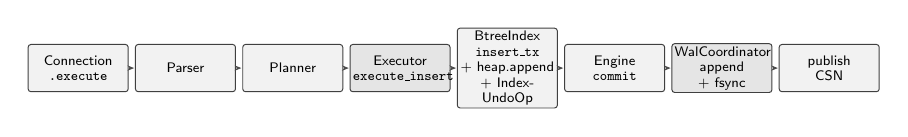
\begin{tikzpicture}[
  font=\sffamily\fontsize{5}{5.6}\selectfont,
  >={Stealth[length=2.4pt,width=1.9pt]},
  every node/.style={inner sep=1pt, line width=0.35pt},
  stage/.style={draw=black!75, line width=0.35pt, rounded corners=1pt,
                fill=black!05, minimum height=6mm, align=center,
                text width=12mm},
  flow/.style={->, draw=black!70, line width=0.35pt, shorten >=0.3pt, shorten <=0.3pt},
]

\node[stage]                    (n1) {Connection\\\texttt{.execute}};
\node[stage, right=0.8mm of n1] (n2) {Parser};
\node[stage, right=0.8mm of n2] (n3) {Planner};
\node[stage, right=0.8mm of n3, fill=black!10]
                                (n4) {Executor\\\texttt{execute\_insert}};
\node[stage, right=0.8mm of n4] (n5) {BtreeIndex\\\texttt{insert\_tx}\\+ heap.append\\+ IndexUndoOp};
\node[stage, right=0.8mm of n5] (n6) {Engine\\\texttt{commit}};
\node[stage, right=0.8mm of n6, fill=black!10]
                                (n7) {WalCoordinator\\append + fsync};
\node[stage, right=0.8mm of n7] (n8) {publish\\CSN};

\foreach \a/\b in {n1/n2, n2/n3, n3/n4, n4/n5, n5/n6, n6/n7, n7/n8} {
  \draw[flow] (\a.east) -- (\b.west);
}

\end{tikzpicture}
\end{document}
